
\clearpage

\section{Explorando a PDB4DNA}
\label{sec:MODIFI}

Deposición de energía/partículas anteriores graficas gnuplot.
energía bases?

\begin{figure}
\centering
\begin{subfigure}{.5\textwidth}
  \centering
  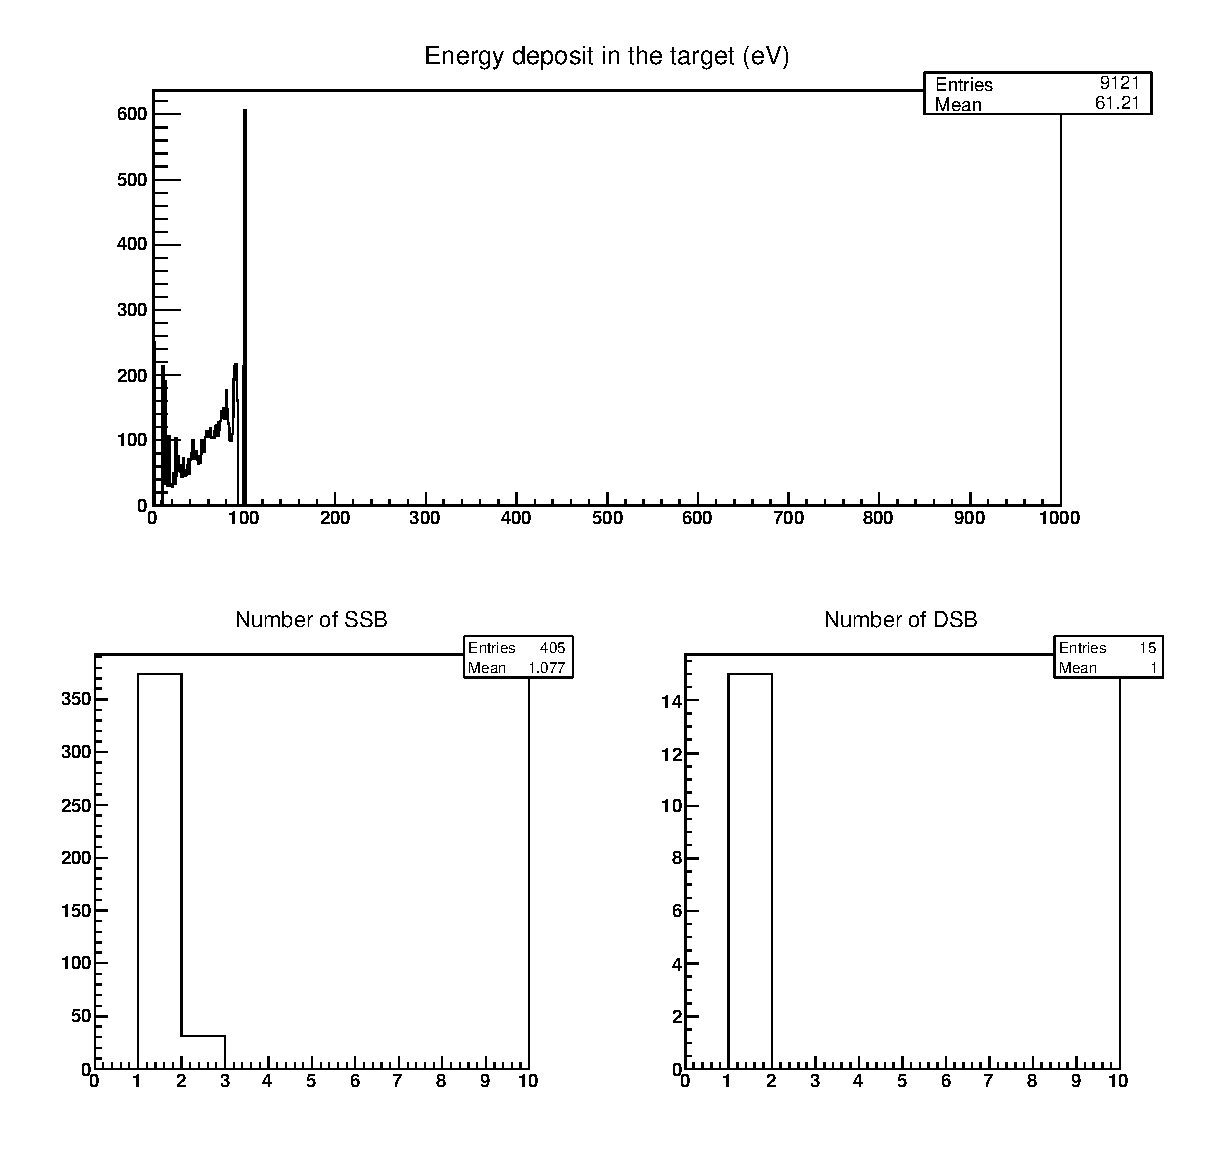
\includegraphics[width=.78\linewidth]{./Figures/e-100ev.eps}
  \caption{100 eV}
  \label{fig:sube1}
\end{subfigure}%
\begin{subfigure}{.5\textwidth}
  \centering
  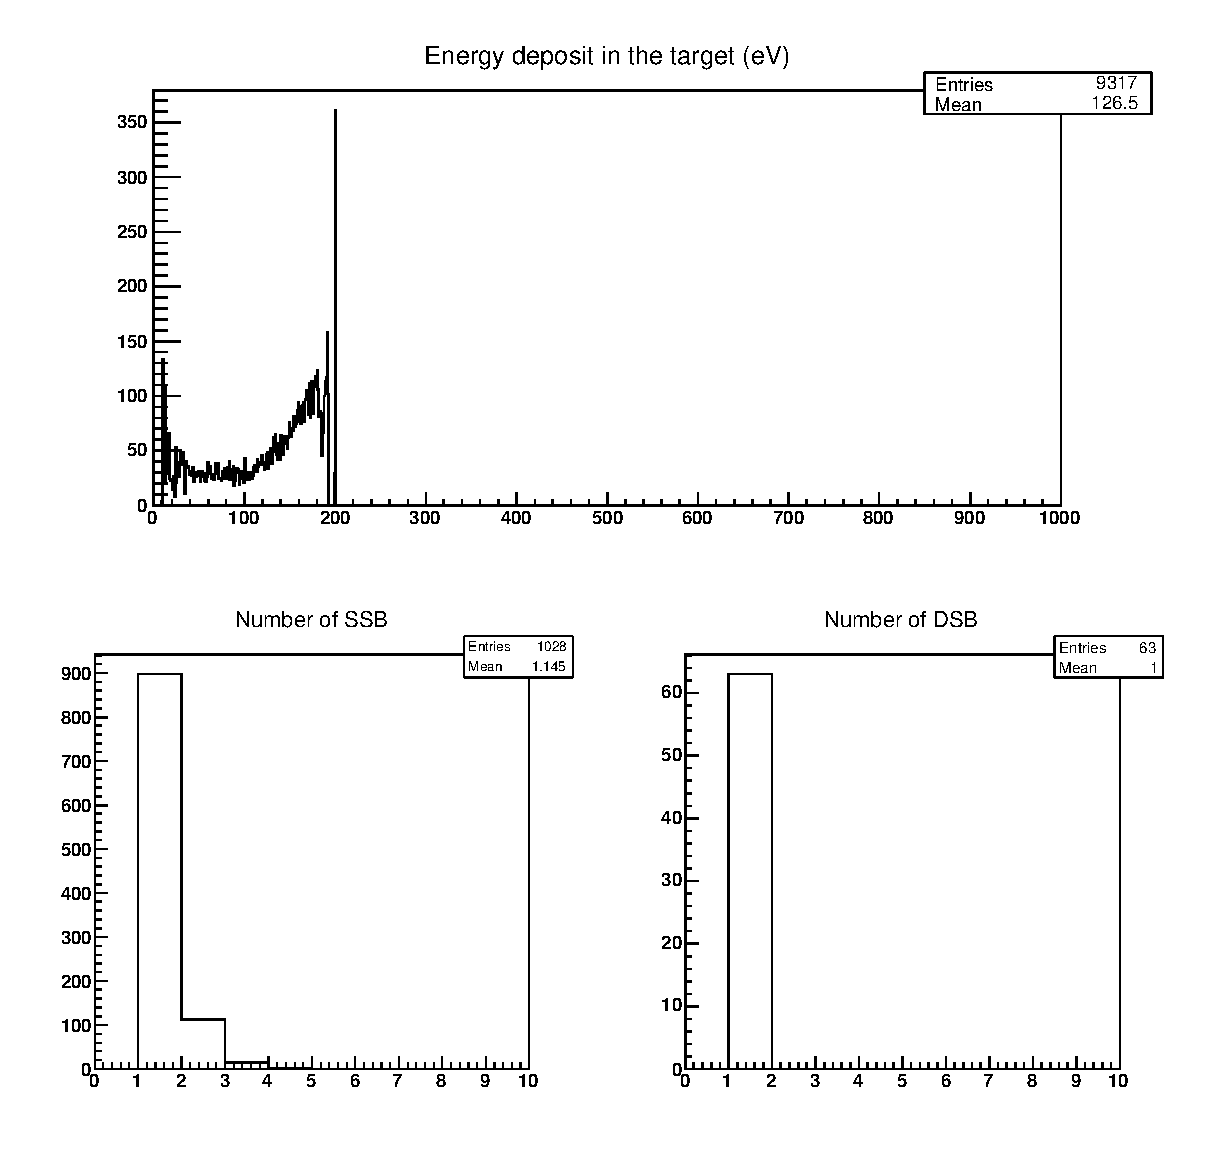
\includegraphics[width=.78\linewidth]{./Figures/e-200ev.eps}
  \caption{200 eV}
  \label{fig:sube2}
\end{subfigure}
\begin{subfigure}{.5\textwidth}
  \centering
  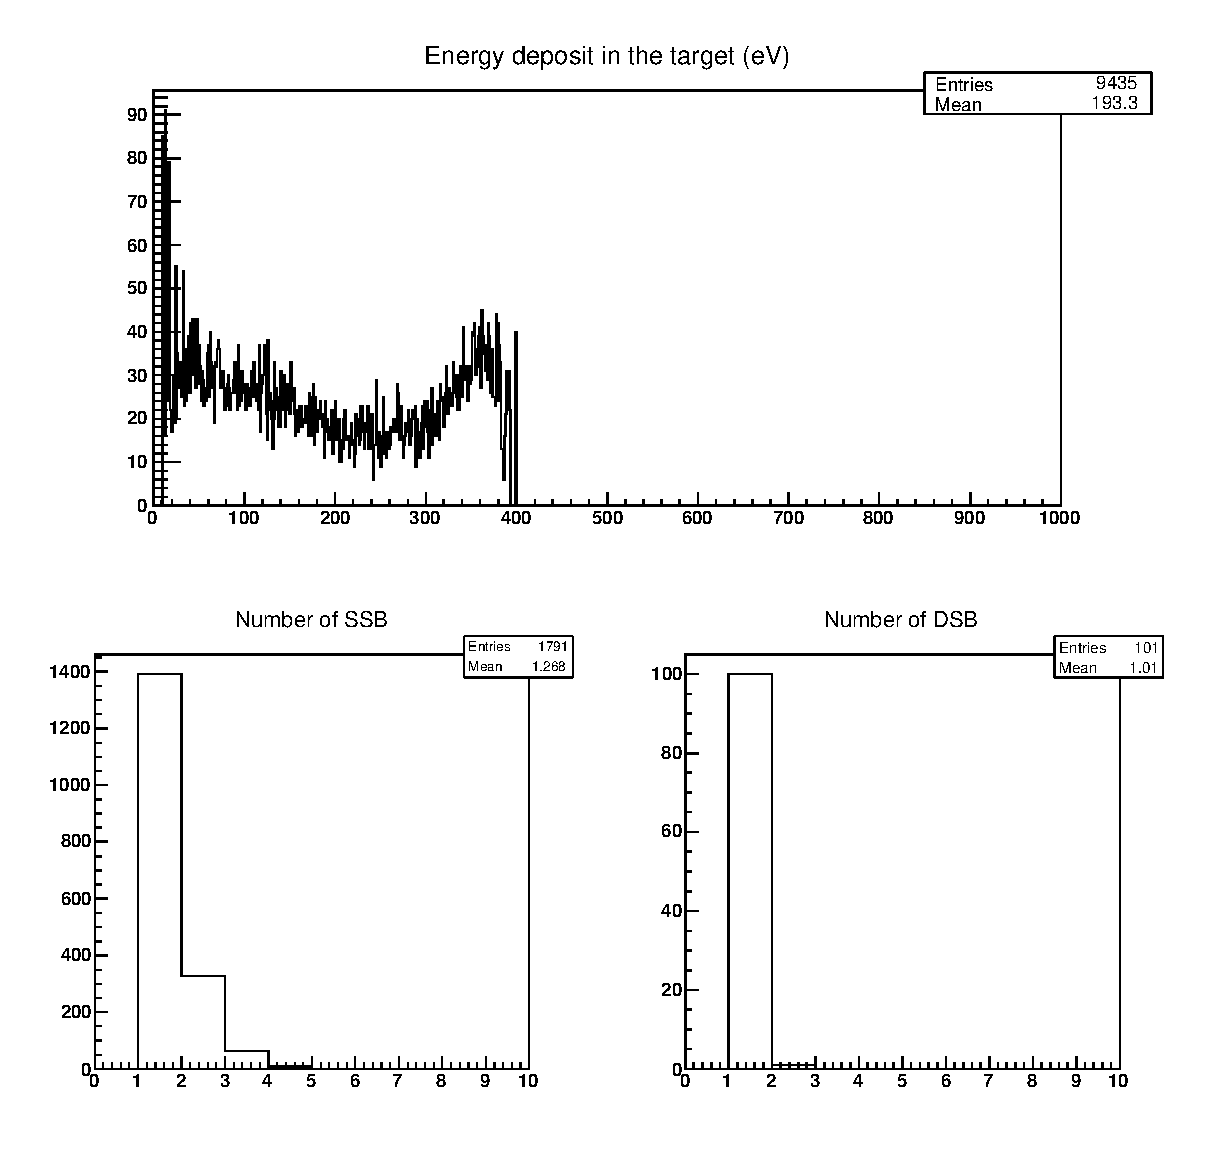
\includegraphics[width=.78\linewidth]{./Figures/e-400ev.eps}
  \caption{400 eV}
  \label{fig:sube3}
\end{subfigure}%
\begin{subfigure}{.5\textwidth}
  \centering
  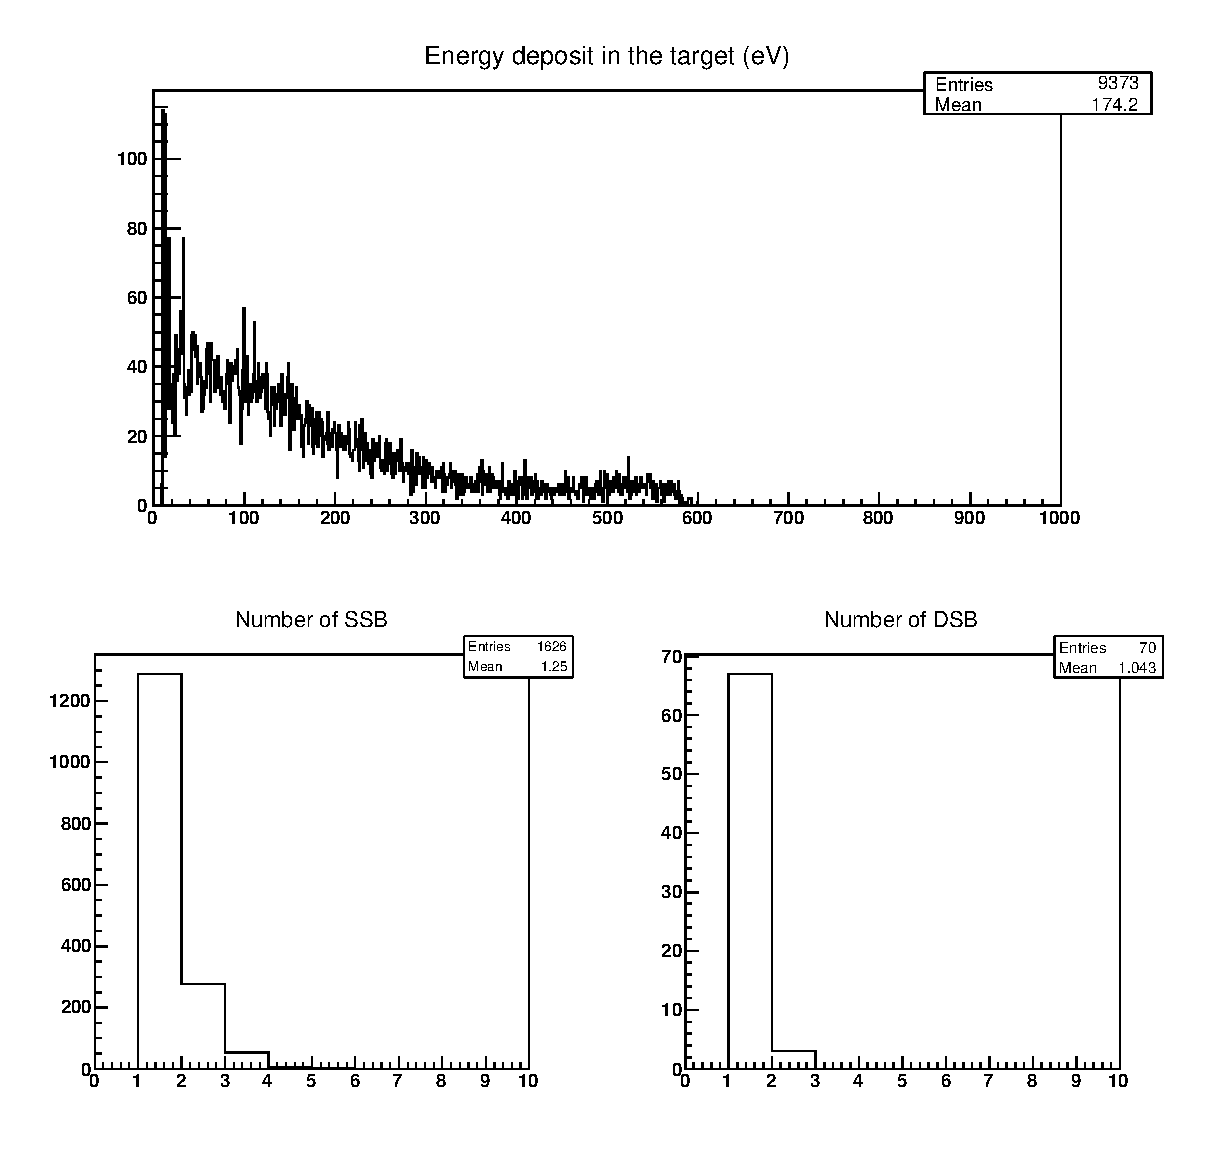
\includegraphics[width=.78\linewidth]{./Figures/e-600.eps}
  \caption{600 eV}
  \label{fig:sube4}
\end{subfigure}
\begin{subfigure}{.5\textwidth}
  \centering
  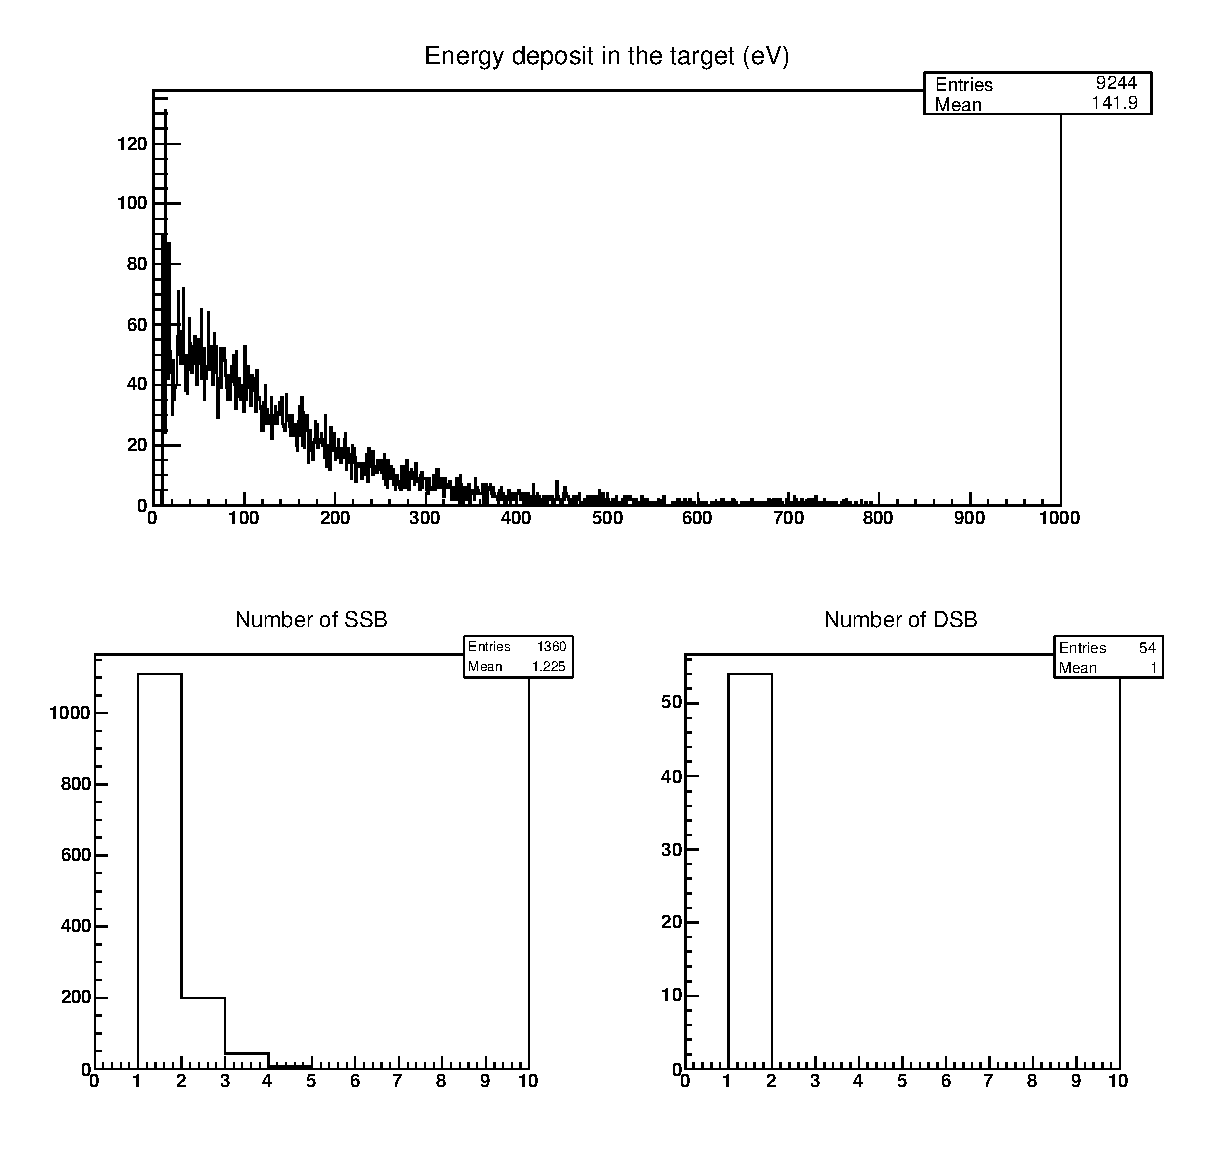
\includegraphics[width=.78\linewidth]{./Figures/e-800ev.eps}
  \caption{800 eV}
  \label{fig:sube5}
\end{subfigure}%
\begin{subfigure}{.5\textwidth}
  \centering
  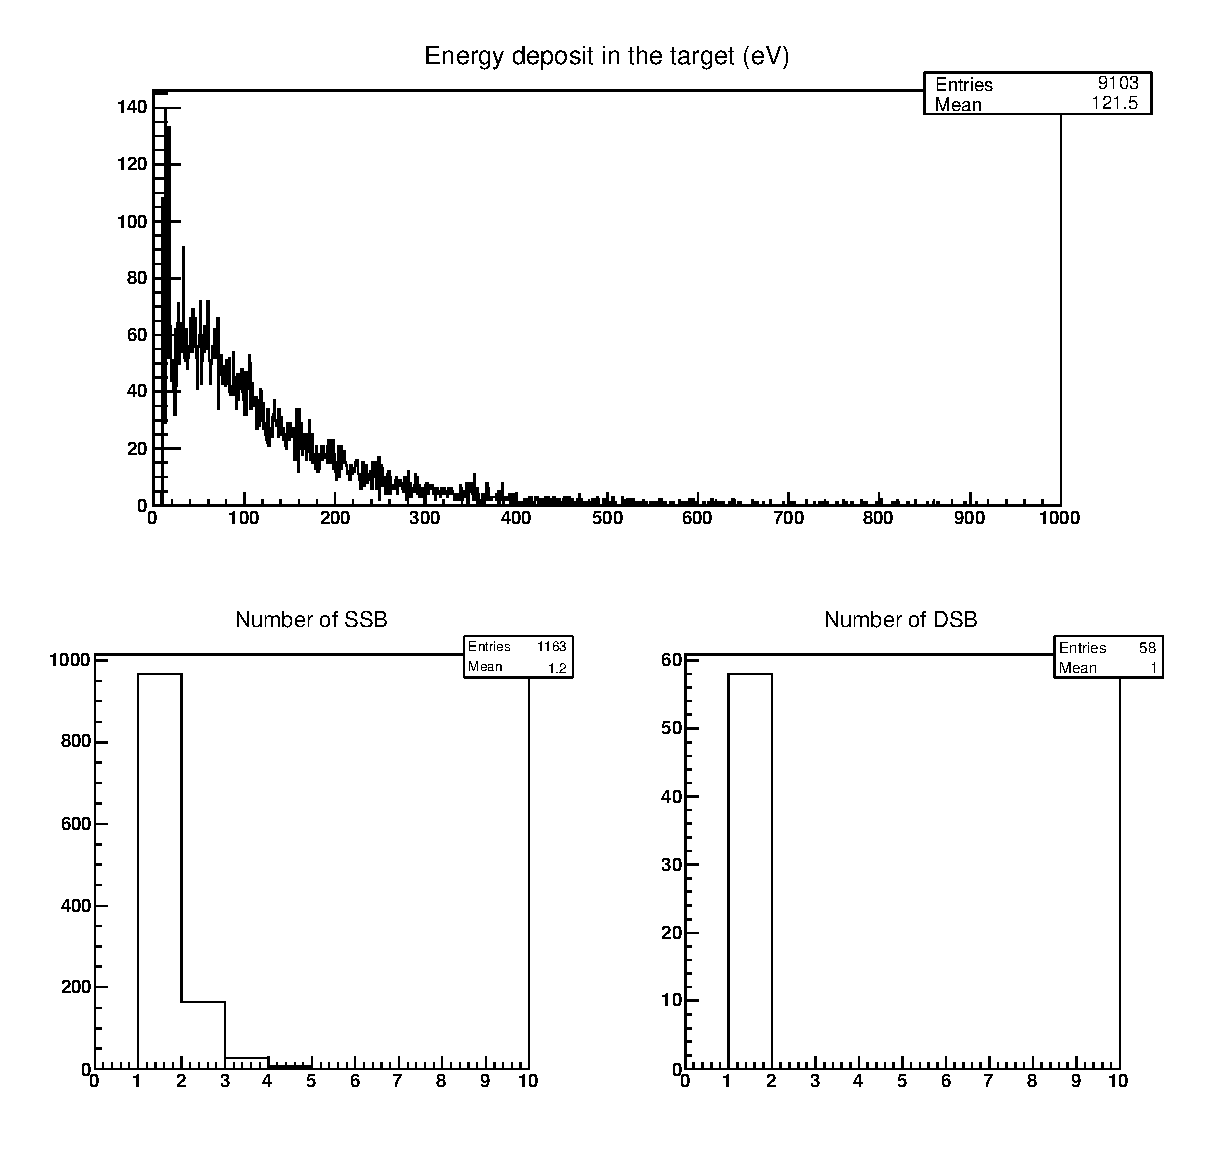
\includegraphics[width=.78\linewidth]{./Figures/e1kev.eps}
  \caption{1 keV}
  \label{fig:sube6}
\end{subfigure}
\begin{subfigure}{.5\textwidth}
  \centering
  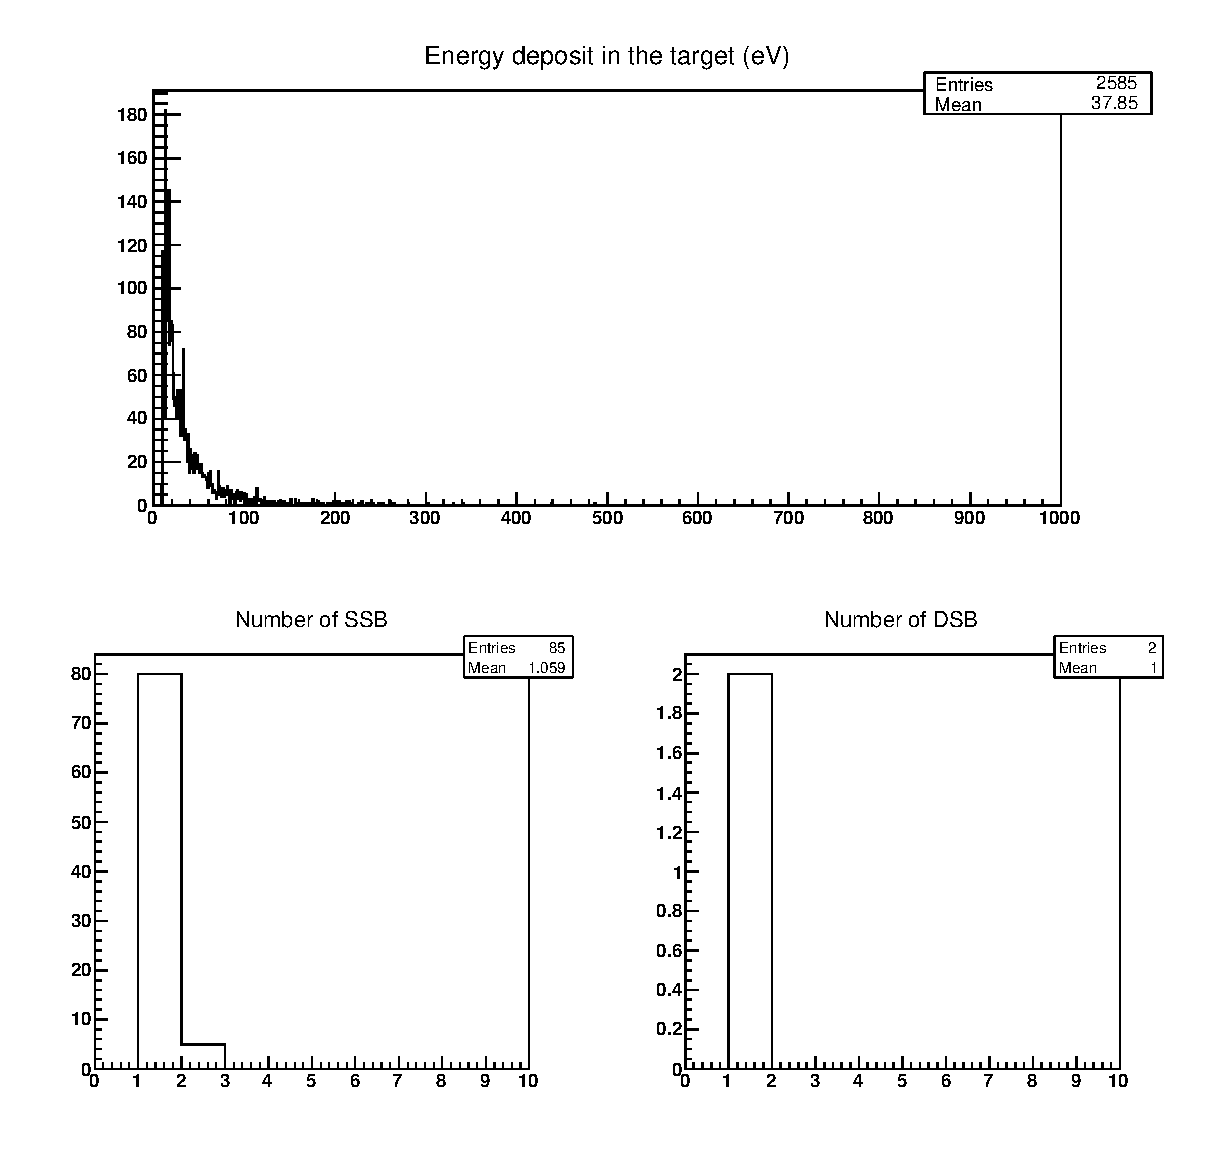
\includegraphics[width=.78\linewidth]{./Figures/e20kev.eps}
  \caption{20 keV}
  \label{fig:sube7}
\end{subfigure}%
\begin{subfigure}{.5\textwidth}
  \centering
  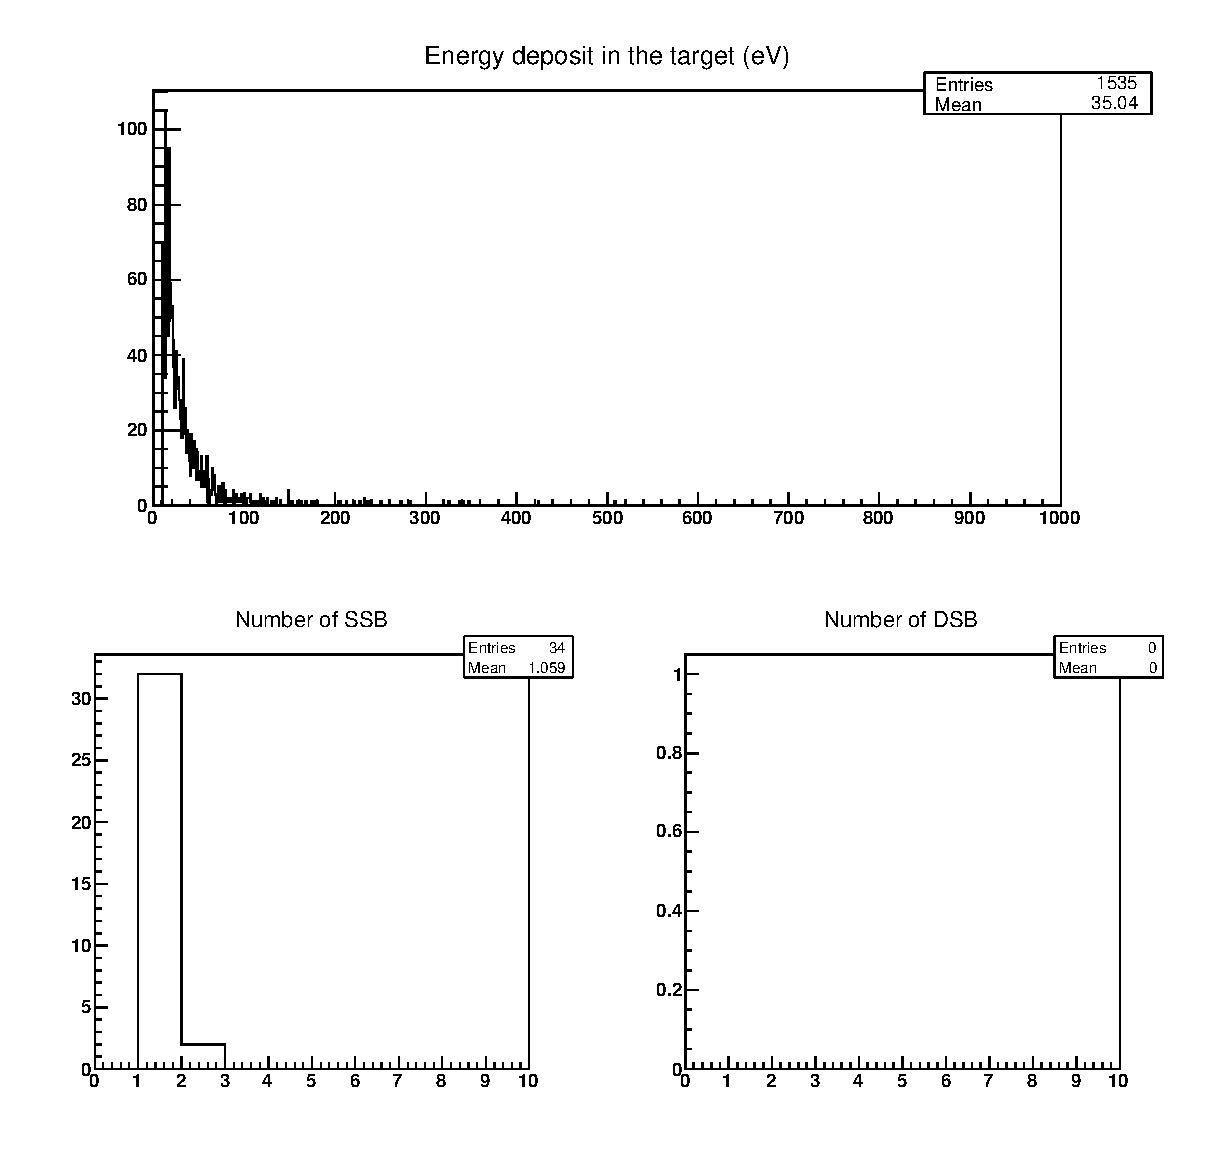
\includegraphics[width=.78\linewidth]{./Figures/e40kev.eps}
  \caption{40 keV}
  \label{fig:sube8}
\end{subfigure}
\caption[Rompimientos simples y dobles electrón(e-)]{Rompimientos simples y dobles electrón(e-)}
\label{fig:e}
\end{figure}

\begin{figure}
\centering
\begin{subfigure}{.5\textwidth}
  \centering
  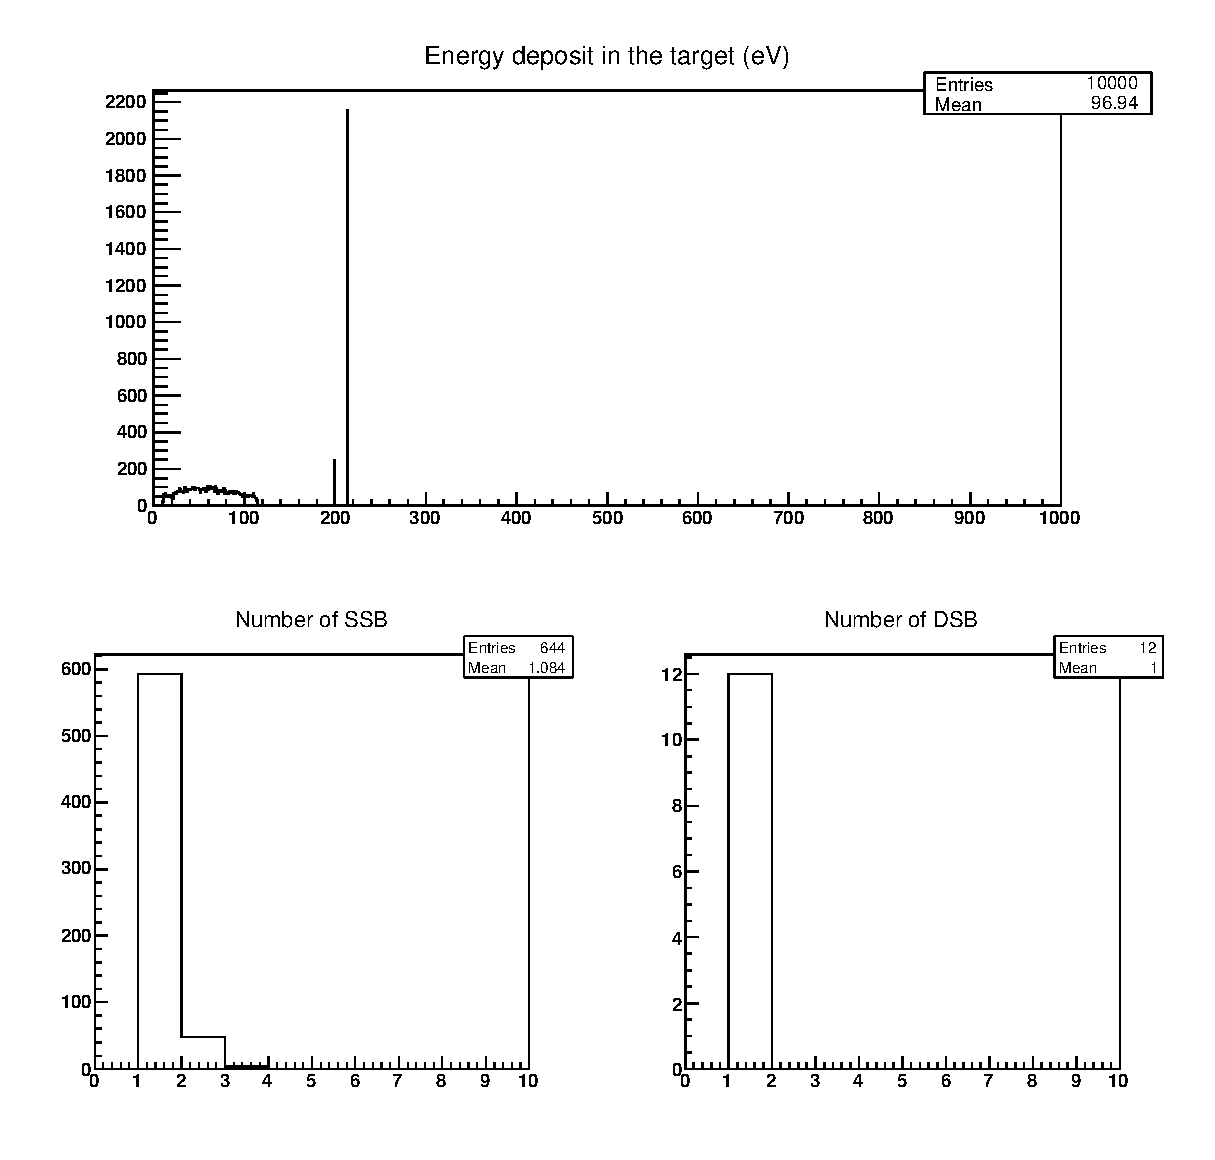
\includegraphics[width=.78\linewidth]{./Figures/proton200eV.eps}
  \caption{200 eV}
  \label{fig:sub1}
\end{subfigure}%
\begin{subfigure}{.5\textwidth}
  \centering
  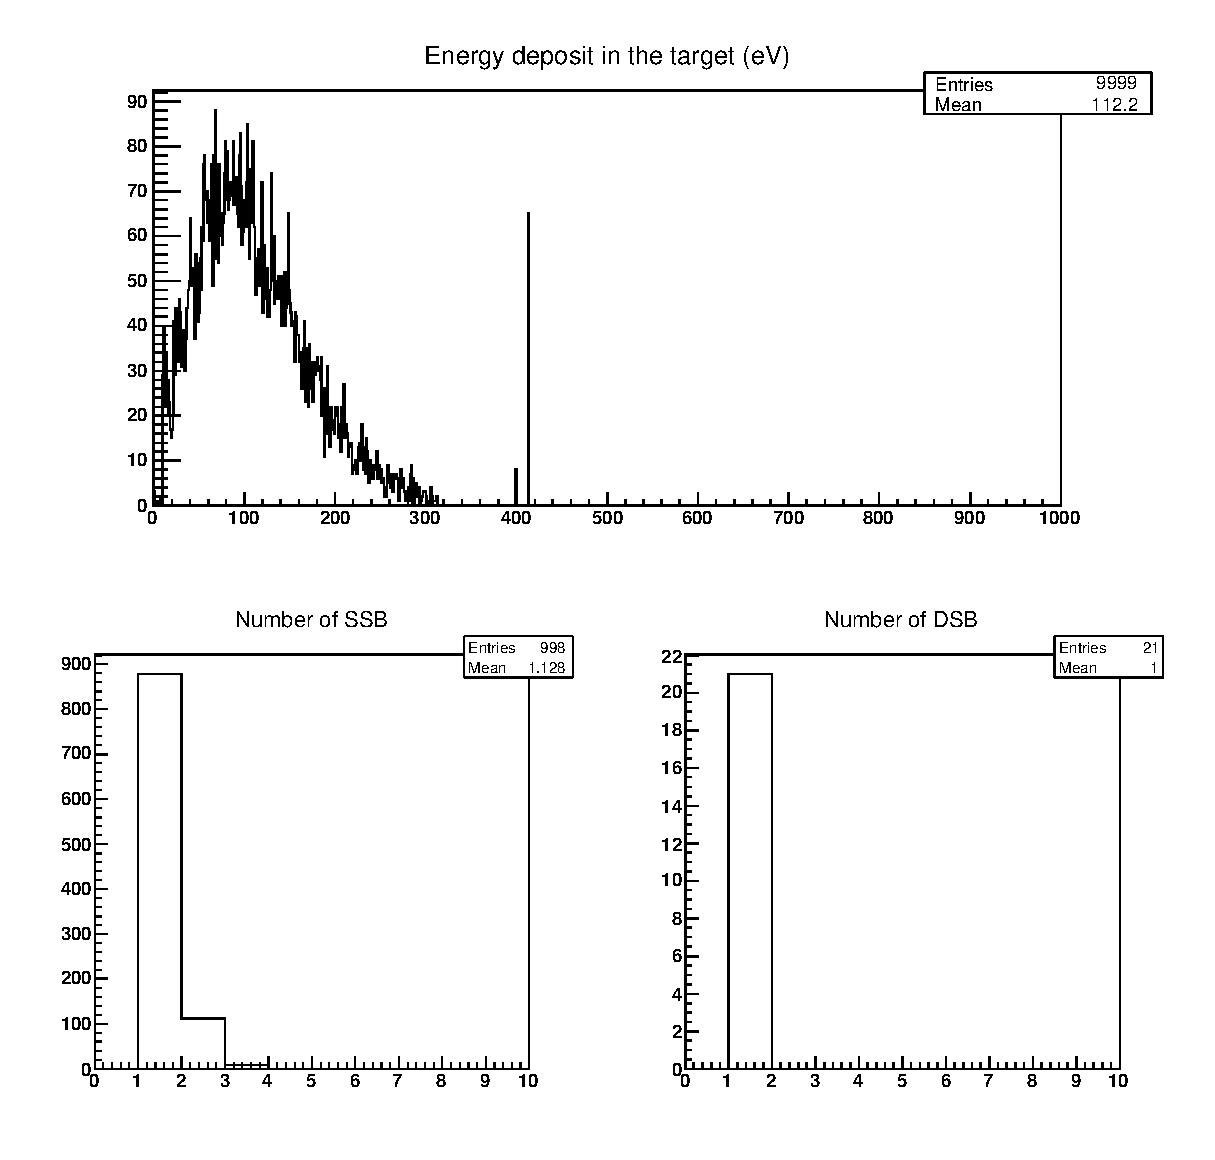
\includegraphics[width=.78\linewidth]{./Figures/proton400eV.eps}
  \caption{400 eV}
  \label{fig:sub2}
\end{subfigure}
\begin{subfigure}{.5\textwidth}
  \centering
  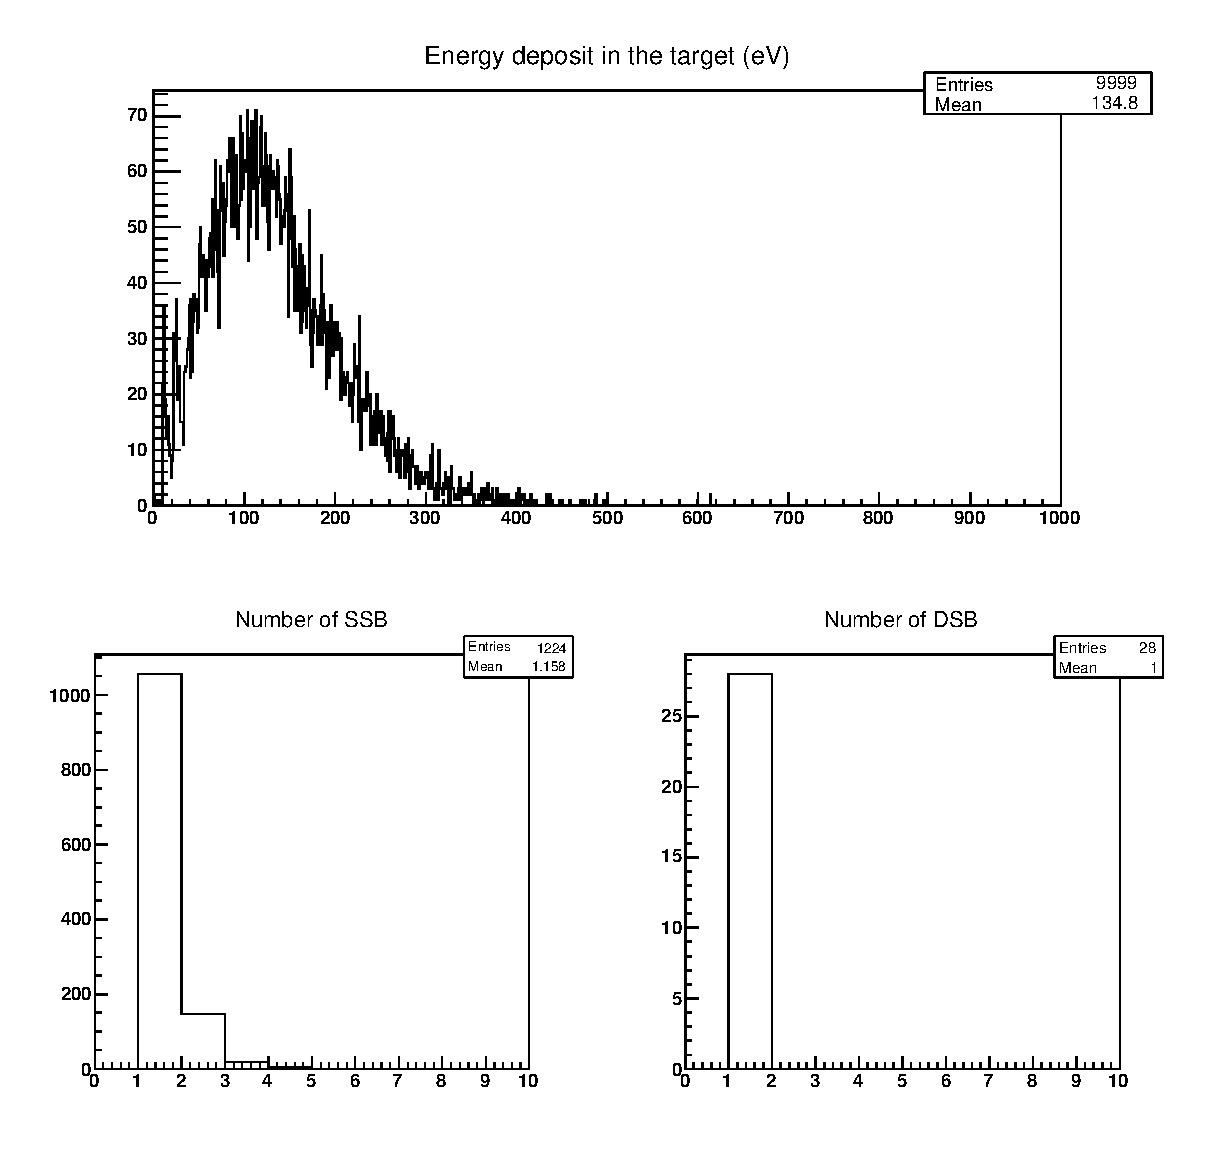
\includegraphics[width=.78\linewidth]{./Figures/proton600eV.eps}
  \caption{600 eV}
  \label{fig:sub3}
\end{subfigure}%
\begin{subfigure}{.5\textwidth}
  \centering
  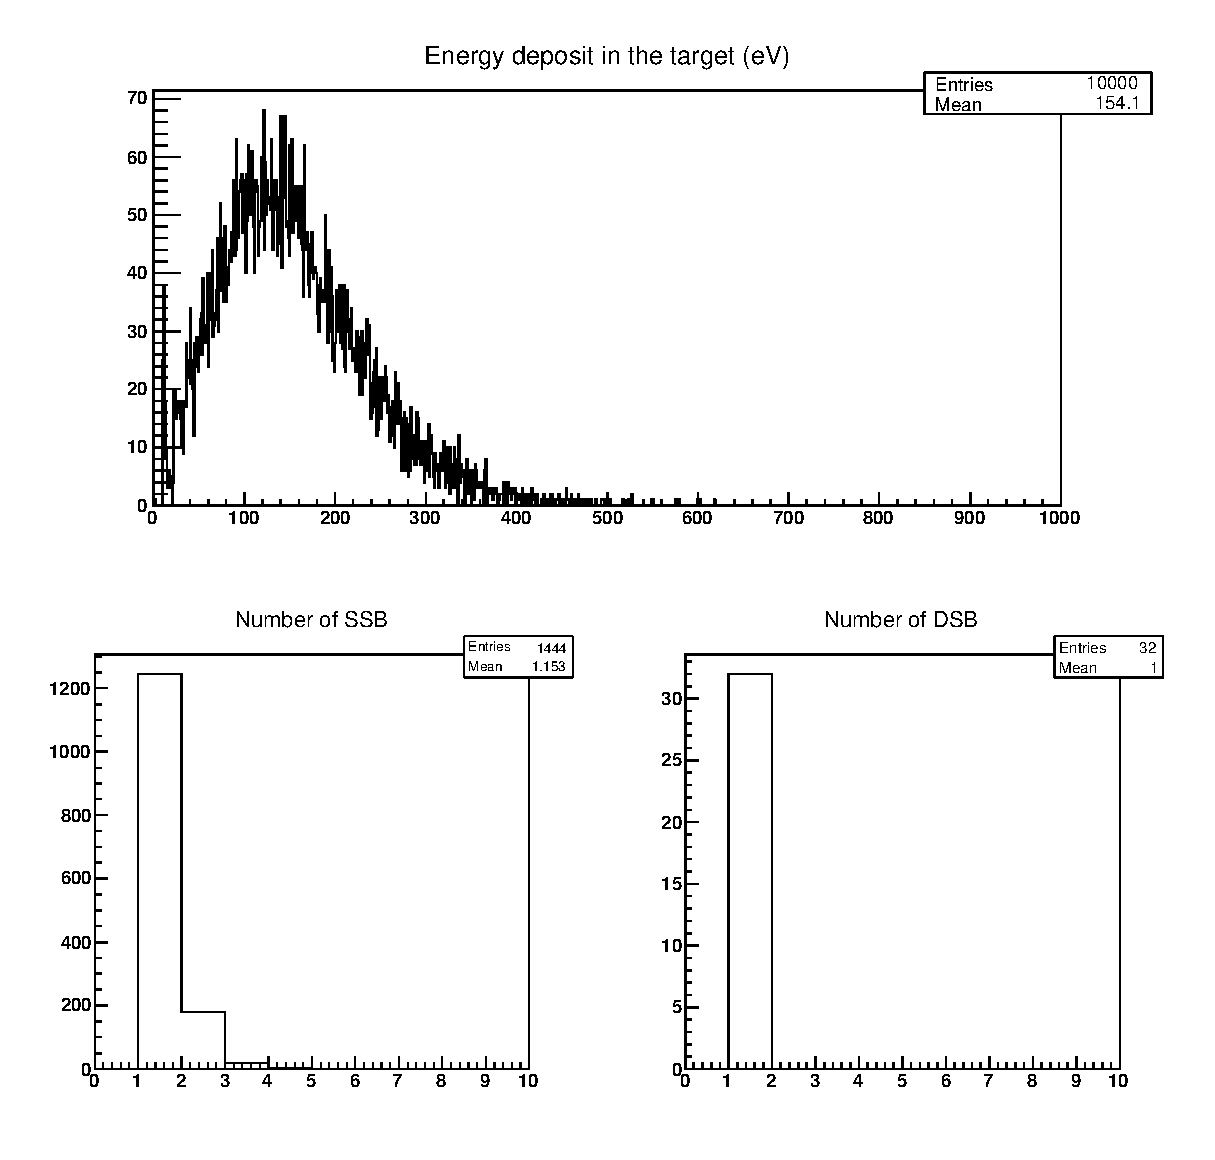
\includegraphics[width=.78\linewidth]{./Figures/proton800eV.eps}
  \caption{800 eV}
  \label{fig:sub4}
\end{subfigure}
\begin{subfigure}{.5\textwidth}
  \centering
  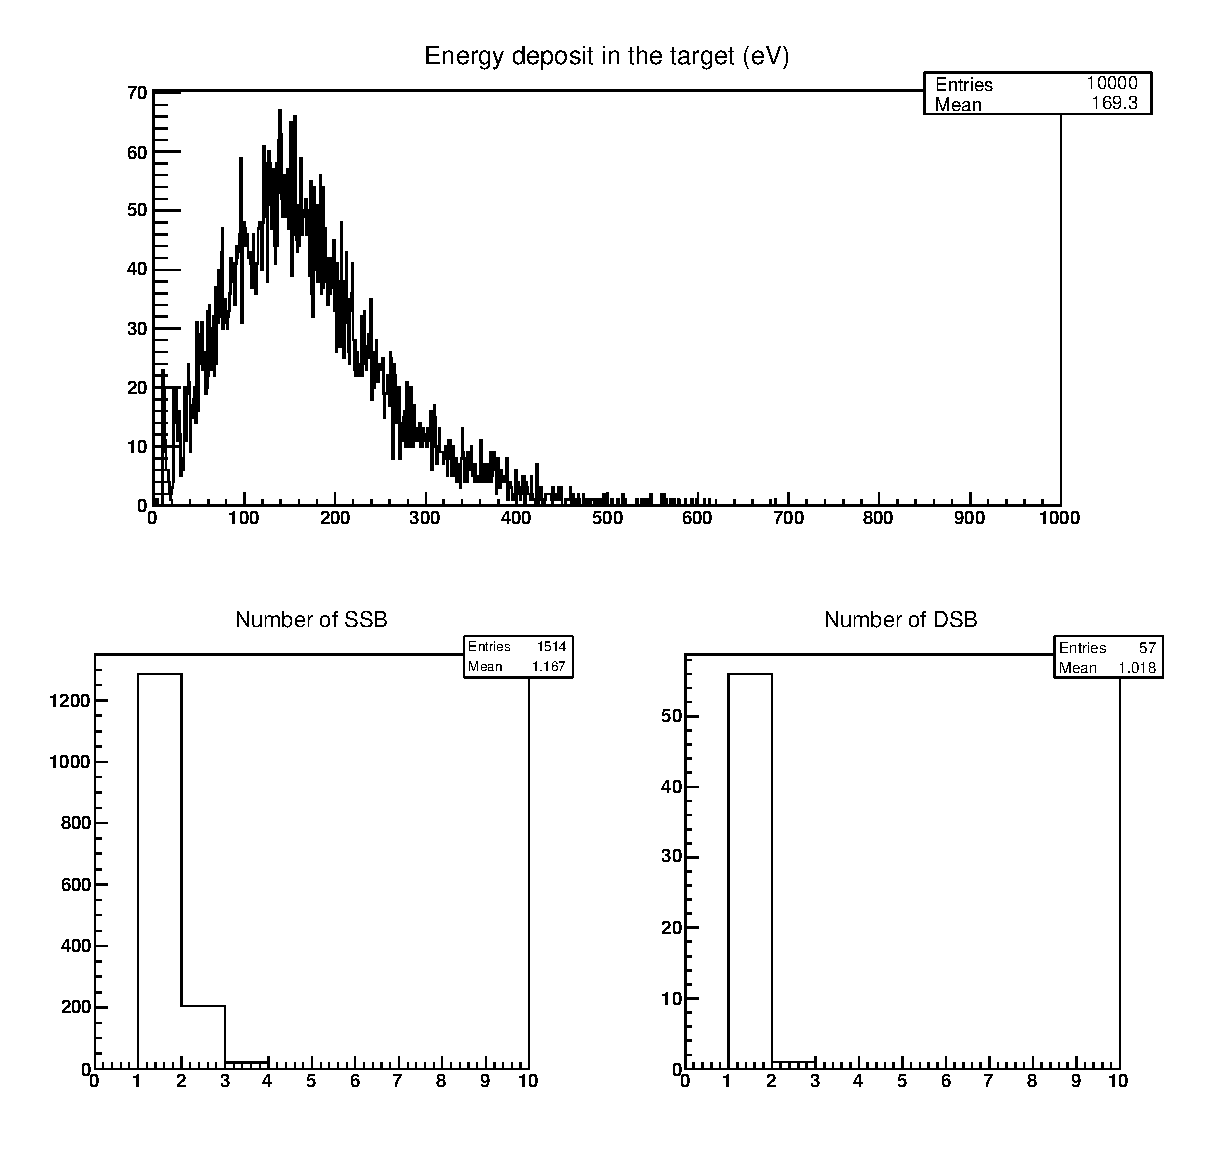
\includegraphics[width=.78\linewidth]{./Figures/proton1kev.eps}
  \caption{1 keV}
  \label{fig:sub5}
\end{subfigure}%
\begin{subfigure}{.5\textwidth}
  \centering
  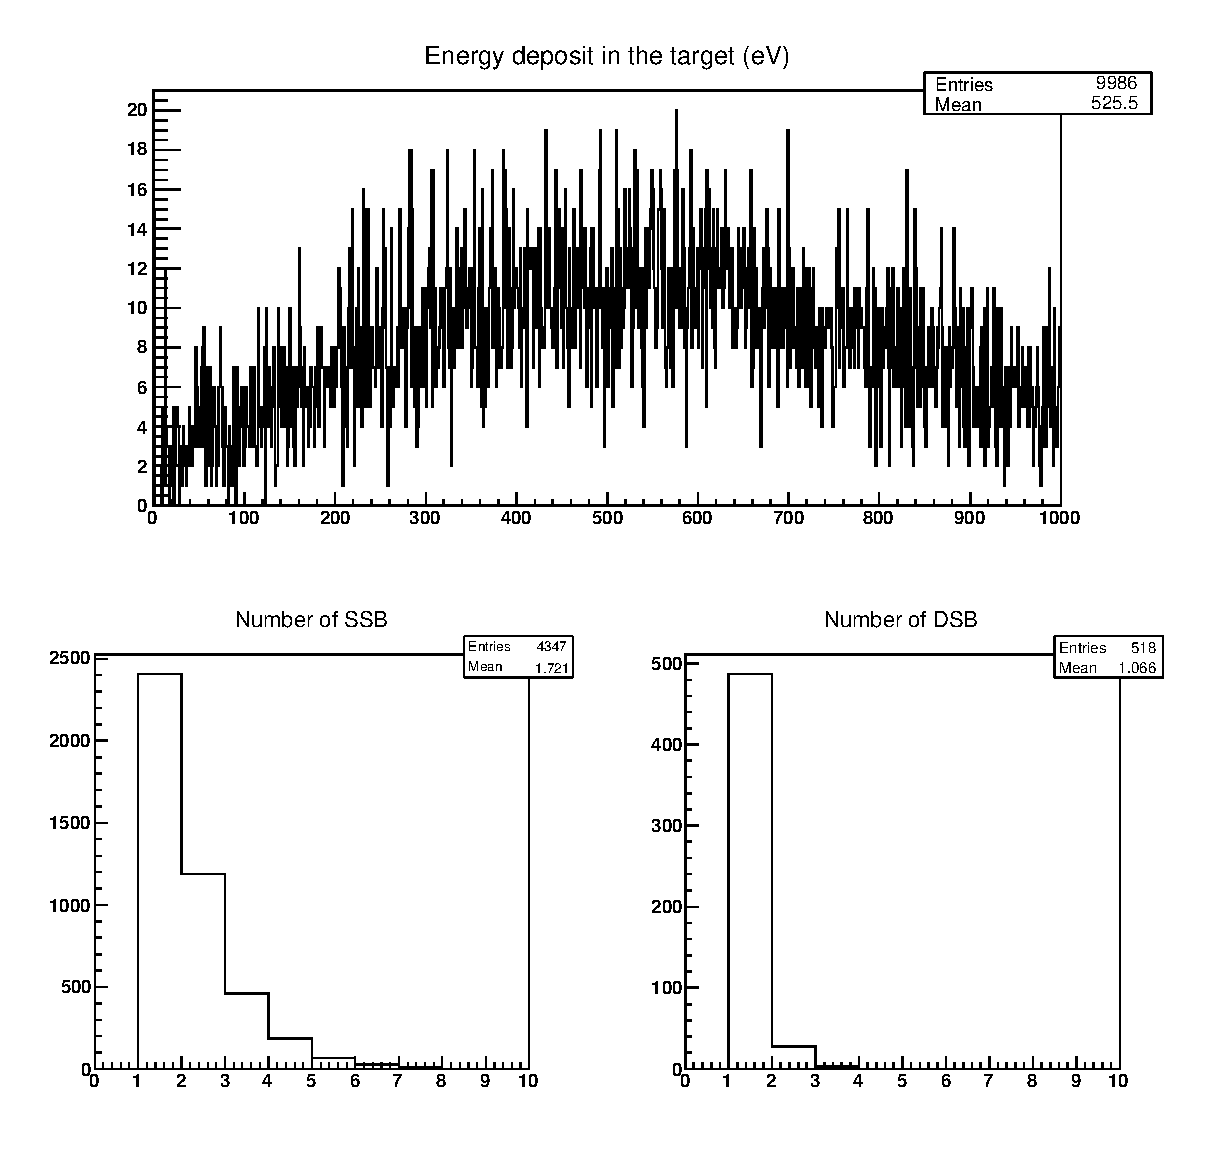
\includegraphics[width=.78\linewidth]{./Figures/proton200kev.eps}
  \caption{200 keV}
  \label{fig:sub6}
\end{subfigure}
\begin{subfigure}{.5\textwidth}
  \centering
  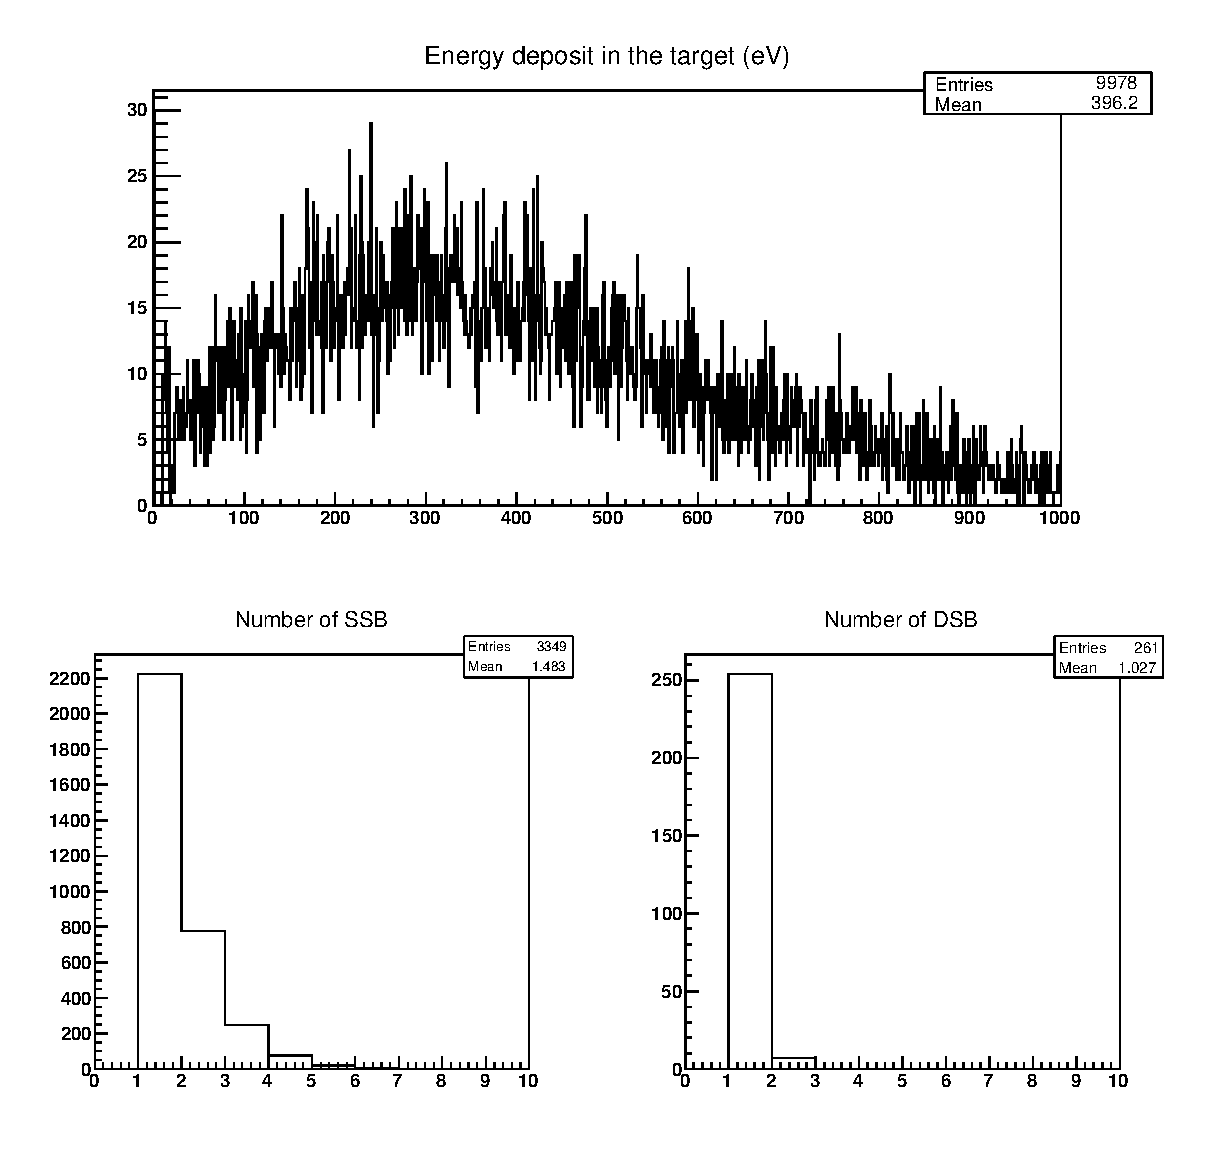
\includegraphics[width=.78\linewidth]{./Figures/proton400kev.eps}
  \caption{400 keV}
  \label{fig:sub7}
\end{subfigure}%
\begin{subfigure}{.5\textwidth}
  \centering
  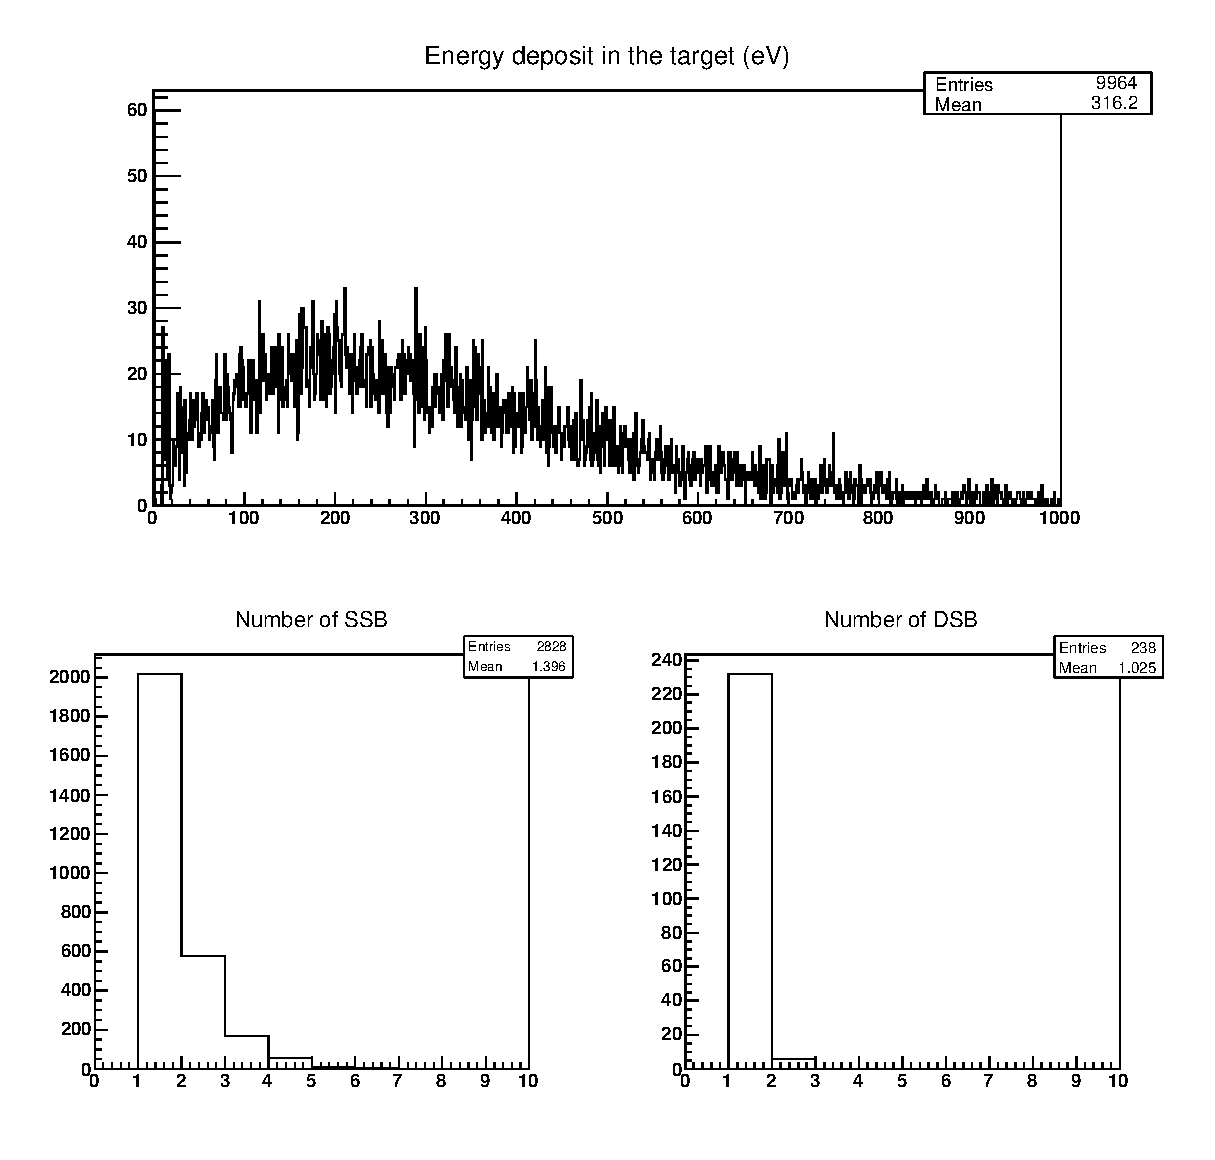
\includegraphics[width=.78\linewidth]{./Figures/proton600kev.eps}
  \caption{600 keV}
  \label{fig:sub8}
\end{subfigure}
\caption[Rompimientos simples y dobles electrón(positron)]{Rompimientos simples y dobles baryon(positron)}
\label{fig:p}
\end{figure}

\begin{figure}
\centering
\begin{subfigure}{.5\textwidth}
  \centering
  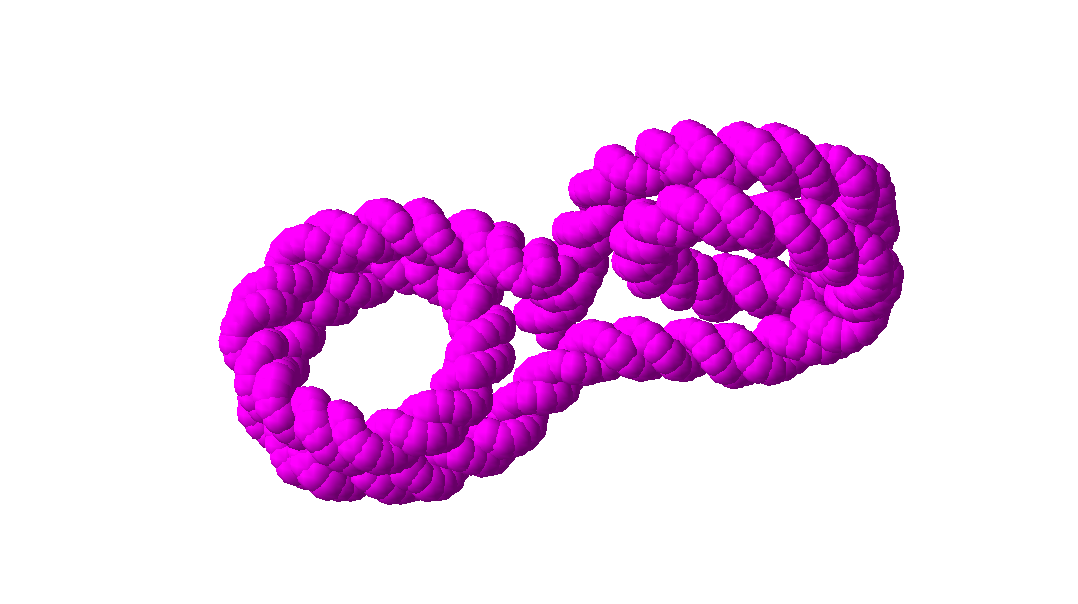
\includegraphics[width=.78\linewidth]{./Figures/a.png}
  \caption{Barycentros}
  \label{fig:su1}
\end{subfigure}%
\begin{subfigure}{.5\textwidth}
  \centering
  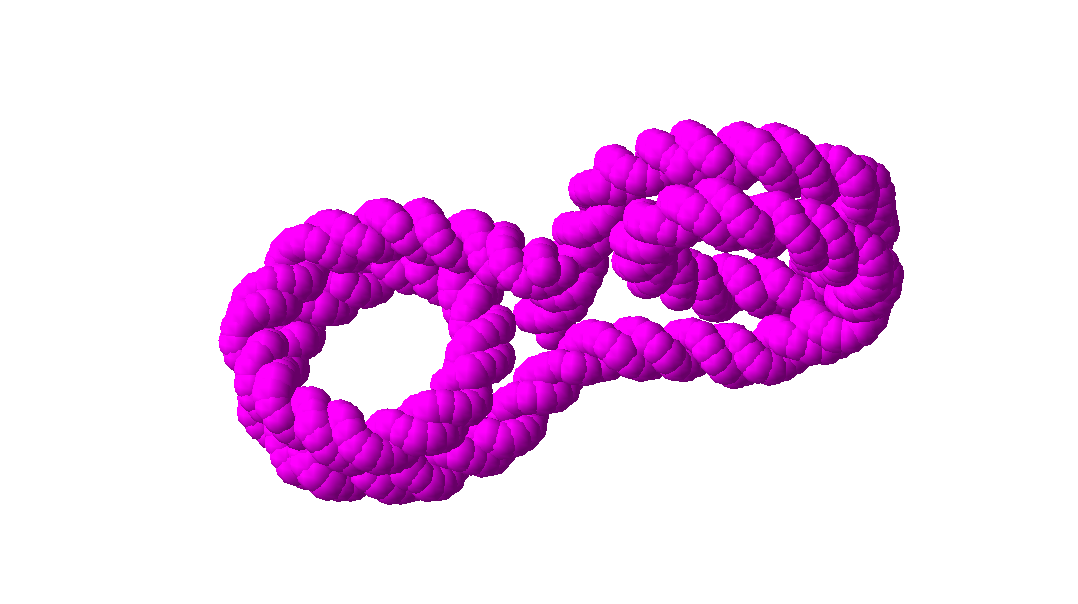
\includegraphics[width=.78\linewidth]{./Figures/a.png}
  \caption{Centros de masa}
  \label{fig:su2}
\end{subfigure}
\caption{Comparación barycentros y centros de masa en Geant4}
\label{fig:test3}
\end{figure}


\begin{figure}[htbp]
    \centering
    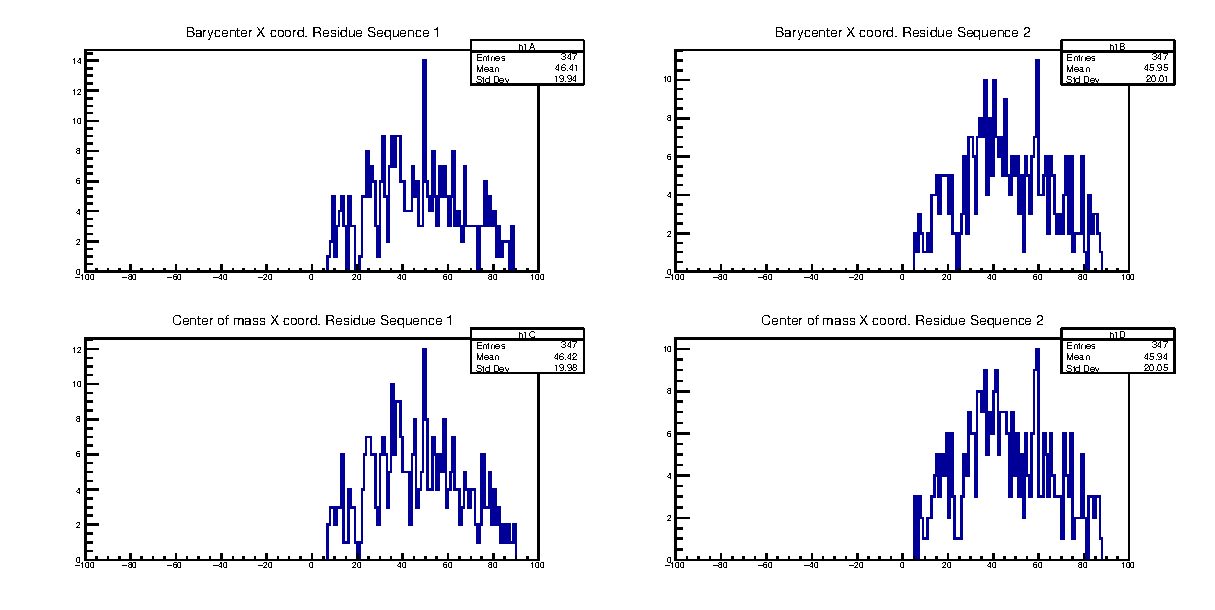
\includegraphics[width=1\linewidth]{./Figures/can1.eps}
    \caption[Barycentros vs centros de masa en x]{Barycentros vs centros de masa en x} % se puede realizar grafico en vmd}
    \label{fig:canx}
\end{figure}

\begin{figure}[htbp]
    \centering
    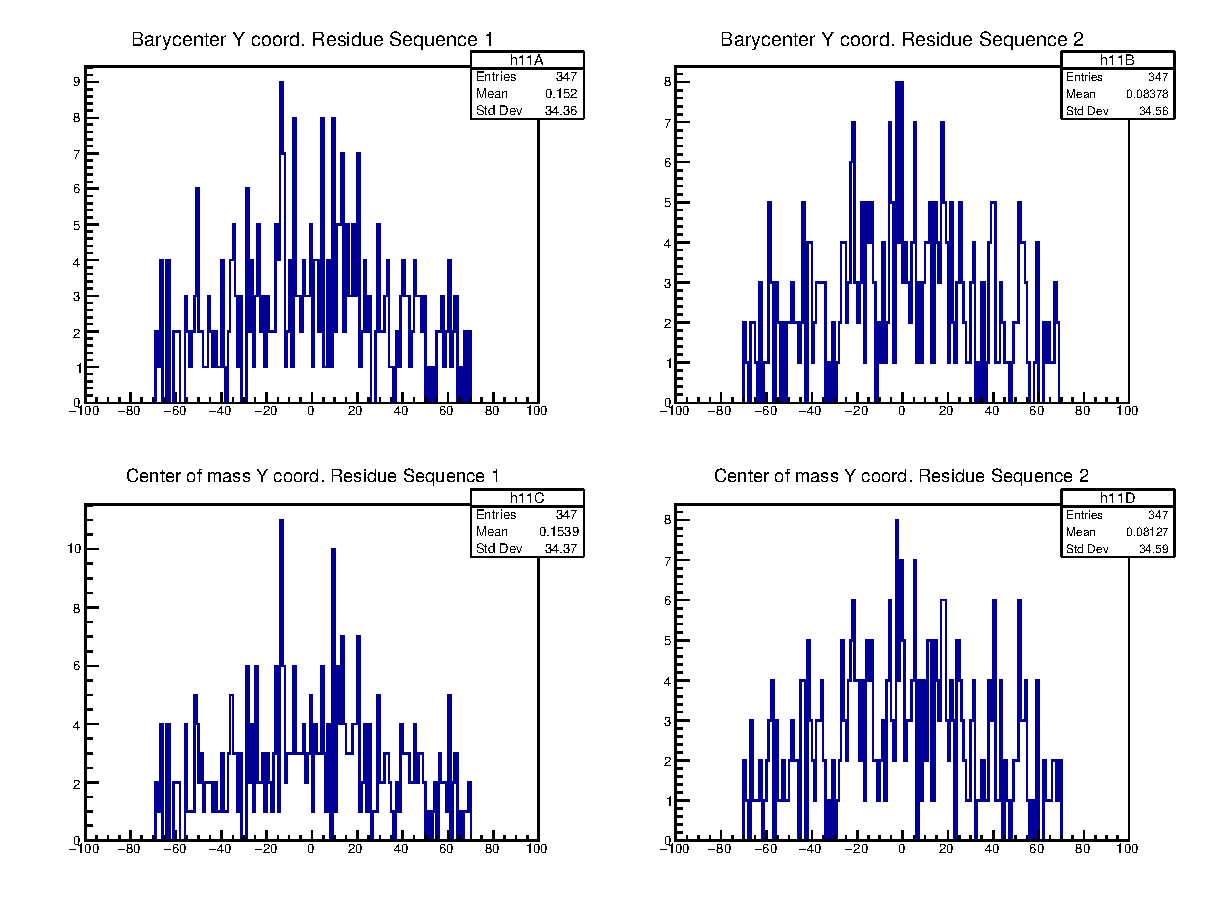
\includegraphics[width=1\linewidth]{./Figures/can2.eps}
    \caption[Barycentros vs centros de masa en y]{Barycentros vs centros de masa en y}
    \label{fig:cany}
\end{figure}

\begin{figure}[htbp]
    \centering
    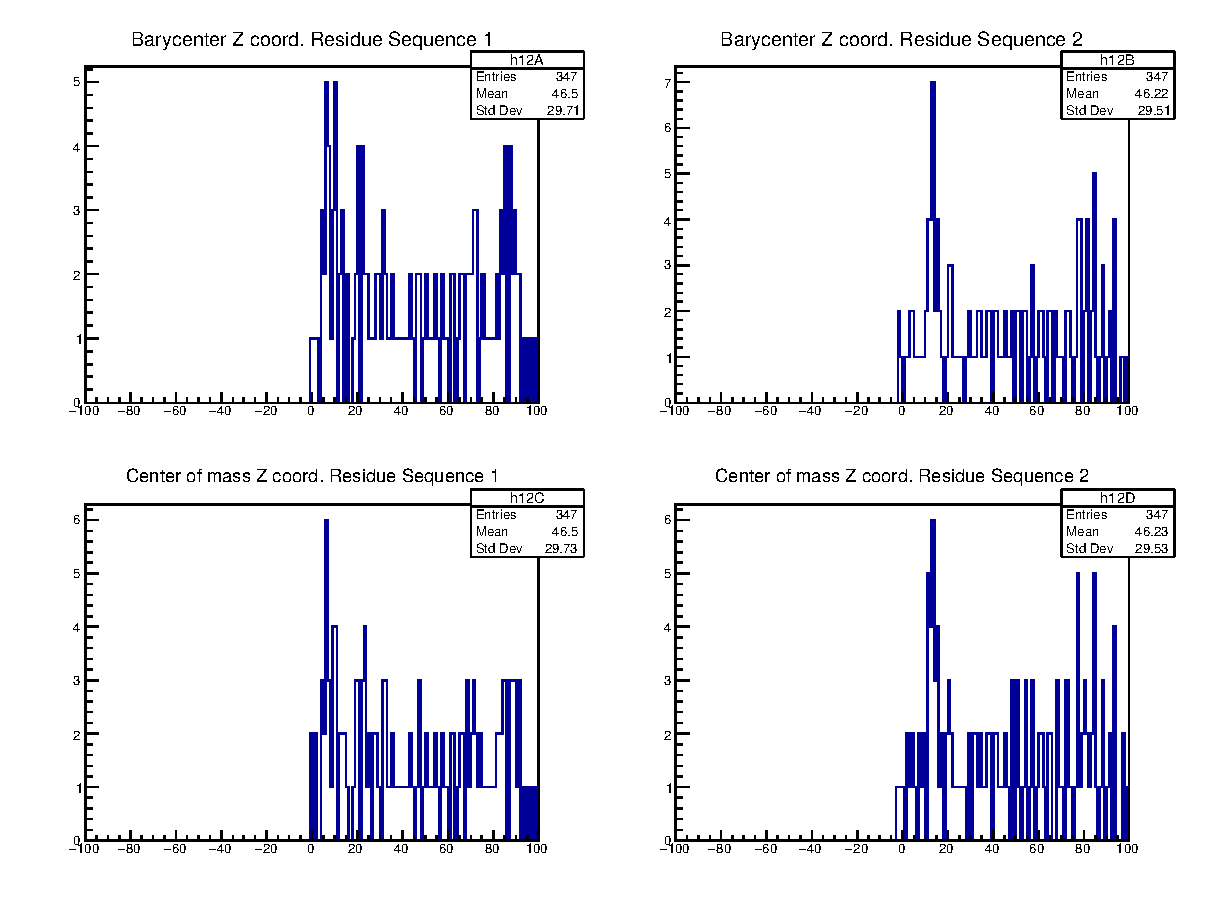
\includegraphics[width=1\linewidth]{./Figures/can3.eps}
  \caption[Barycentros vs centros de masa en z]{Barycentros vs centros de masa en z}
    \label{fig:canz}
\end{figure}


hablar algo de TER Y limitaciones
Hacer modificaciones de TER
mismas particulas?
centros de masa
PDB4DNA fue modificado de tal manera que en vez de hacer uso de las esferas ligadas a partir de barycentros usara centros de masa, para esto se uso el archivo PDBlib, primero se definió la masa de los diferentes elementos (véase anexo ~\ref{app:A}),y luego se usaron las clases bases ya definidas en PDBlib para hacer los respectivos cálculos de centros de masa(véase anexo ~\ref{app:B}).\\
